\documentclass[10pt,letterpaper]{article}

\usepackage[margin=0.7in]{geometry}
\usepackage[utf8]{inputenc}
\usepackage[T1]{fontenc}
\usepackage{lmodern}
\usepackage{microtype}
\usepackage{amsmath, amssymb, amsthm}
\usepackage{mathtools}
\usepackage{bm}
\usepackage{booktabs}
\usepackage{array}
\usepackage{graphicx}
\usepackage{caption}
\usepackage{subcaption}
\usepackage{float}
\usepackage[hidelinks]{hyperref}
\usepackage{xcolor}
\usepackage{csquotes}
\usepackage[authoryear,round]{natbib}
\usepackage{titlesec}
\usepackage{multicol}

\titlespacing*{\section}{0pt}{0.8ex plus 0.3ex}{0.4ex plus 0.2ex}
\titlespacing*{\paragraph}{0pt}{0.5ex plus 0.2ex}{0.6em}
\setlength{\parskip}{0.25ex}
\setlength{\parindent}{0pt}
\setlength{\abovecaptionskip}{3pt}
\setlength{\belowcaptionskip}{0pt}
\setlength{\textfloatsep}{6pt plus 1pt minus 1pt}
\setlength{\intextsep}{6pt plus 1pt minus 1pt}
\renewcommand{\arraystretch}{1.05}

\captionsetup{font=small, labelfont=bf, labelsep=period, skip=2pt}

\title{\vspace{-2.5em}Exploiting the Errors, Revisited: HARQ Volatility Forecasting\\[-0.15em] with Signed-Jump Decomposition and Probabilistic Extensions}
\author{Aprameya Tirupati\\\small Georgia Institute of Technology $\cdot$ GTSF IC Quant Mentorship, Spring 2026}
\date{\vspace{-1em}}

\begin{document}
\maketitle
\vspace{-3.5em}

\section*{Overview}
Volatility --- how much a financial asset's price swings day to day --- is a central input to risk management, portfolio allocation, and option pricing, so forecasting tomorrow's volatility is a question many billions of dollars depend on. A widely-cited 2016 paper by \citet{bpq2016} proposed a simple correction to the standard volatility-forecasting model, claiming a 5--10\% accuracy gain; this project revisits that claim on the authors' own data and asks three questions. First, does the correction still work a decade after publication? Second, can it be usefully combined with a related improvement from \citet{pattonsheppard2015} that distinguishes up-move volatility from down-move volatility? Third, can a modern machine-learning method produce not just a point forecast but a full probability distribution for next-day volatility --- the kind of output a risk manager actually needs? The correction works decisively on the original data (a 12\%-plus improvement on the competition's preferred accuracy metric); the novel combination improves on it by a further 4.6\%; and the machine-learning extension delivers near-nominal 96.9\% coverage at a 95\% target --- the calibrated probability distributions that risk managers actually need for value-at-risk. The remainder of this document presents the methodology and detailed results.

\section{Introduction and data}
The heterogeneous autoregressive (HAR) model of \citet{corsi2009},
\begin{equation}
RV_{t+1} = \beta_0 + \beta_d RV_t + \beta_w RV_t^{(w)} + \beta_m RV_t^{(m)} + \varepsilon_{t+1},
\end{equation}
has been the volatility-forecasting workhorse for two decades. \citet{bpq2016} (hereafter BPQ) augment HAR with a measurement-error term proportional to $\sqrt{RQ_t}$; \citet{pattonsheppard2015} decompose $RV$ into positive and negative semivariances $RS^+$, $RS^-$ \citep[following][]{bns2010} and show $\beta_- > \beta_+$ --- bad volatility is more persistent than good.

SPX data are the stitched combination of \texttt{HARModel::SP500RM} \citep[][4{,}096 trading days, 1997-05 to 2013-08]{sjoerup2019} and \texttt{highfrequency::SPYRM} (2014-01 to 2019-12, 1{,}495 days). Both ship $RV$, $RQ$, $BPV$ computed from 5-minute returns. SP500RM additionally ships positive and negative semivariances ($RVp$, $RVn$); SPYRM does not, so SHAR, HARQ-Signed, and NGBoost-HARQ are scoped to the SP500RM portion. The SP500RM date index is reconstructed by anchoring row 2869 ($RV \approx 60.6$) to 2008-10-09 and row 3581 ($RV = 19.55$) to the 2011-08-08 S\&P-downgrade reaction. Crypto data are 1-minute BTCUSDT and ETHUSDT klines from \texttt{data.binance.vision} (198 monthly files, 2018-01 to 2026-03), with all measures computed from 5-minute subsampled returns. NDX, RUT, and DJIA are deliberately excluded because genuine realized quarticity is not publicly distributed for those indices.

\section{Methods}
Six HAR-family baselines (HAR, HAR-J of \citealp{abd2007}, SHAR, HARQ, HARQ-F, CHAR) share a common Python \texttt{VolForecaster} API fit via \texttt{numpy.linalg.lstsq}. HARQ uses the centered interaction
\begin{equation}
RV_{t+1} = \beta_0 + \left(\beta_d + \beta_Q\!\left(\sqrt{RQ_t} - \overline{\sqrt{RQ}}\right)\right) RV_t + \beta_w RV_t^{(w)} + \beta_m RV_t^{(m)} + \varepsilon_{t+1},
\end{equation}
following the \texttt{HARModel} R package convention --- equivalent in prediction to BPQ's uncentered form but numerically better-conditioned. \textbf{HARQ-Signed}, the novel contribution, nests both HARQ and SHAR:
\begin{align}
RV_{t+1} &= \beta_0 + \left(\beta_d + \beta_Q\!\left(\sqrt{RQ_t} - \overline{\sqrt{RQ}}\right)\right) RV_t + \beta_+ RS^+_t + \beta_- RS^-_t + \beta_w RV_t^{(w)} + \beta_m RV_t^{(m)} + \varepsilon_{t+1}.
\end{align}
Walk-forward evaluation is expanding-window, monthly refit, initial 1{,}000-day window, with a BPQ insanity filter that replaces non-positive or extreme non-HAR predictions with the HAR prediction; NaN filtering is \emph{per model} on its feature requirements so HAR / HARQ / HARQ-F / CHAR run on the full SP500RM+SPYRM stitch even though SHAR / HARQ-Signed cannot. Losses are MSE and the QLIKE of \citet{patton2011}, $\mathrm{QLIKE}(y, \hat{y}) = y/\hat{y} - \log(y/\hat{y}) - 1$. Diebold--Mariano tests use Newey--West HAC at bandwidth $h-1$; the Model Confidence Set \citep{hln2011} is computed via \texttt{arch.bootstrap.MCS} with 1{,}000 bootstrap replications. NGBoost-HARQ \citep{ngboost2020} uses a Normal output distribution (\texttt{n\_estimators}=300, \texttt{learning\_rate}=0.01) on features $\{RV_d, RV_w, RV_m, RV_d \cdot (\sqrt{RQ_d}-\overline{\sqrt{RQ}}), BV_d\}$; empirical coverage, CRPS, and Kupiec / Christoffersen VaR tests \citep{kupiec1995,christoffersen1998} evaluate calibration.

\section{Results}
\paragraph{Reproduction (Table~\ref{tab:repro}).} Rolling 1{,}000-day window on SP500RM 2002--2013 at $h = 1$: HAR QLIKE $= 0.1646$ (baseline); SHAR 0.1557 ($-5.40\%$, DM $p = 0.0003$, matches \citealp{pattonsheppard2015}); HARQ 0.1682 QLIKE ($+2.18\%$) and MSE $-4.4\%$ (matches BPQ direction on MSE); HAR-J and CHAR tie HAR; HARQ-F is unstable under plain OLS and only becomes competitive after the insanity filter.

\begin{table}[tb]
\centering\small
\caption{Reproduction of \citet{bpq2016} Table 3 on SP500RM, rolling-1{,}000-day window, $h=1$, 2002--2013. QLIKE deltas and Diebold--Mariano $p$-values against HAR; MSE in units of $10^{-8}$.}
\label{tab:repro}
\begin{tabular}{lrrrrr}
\toprule
Model & QLIKE & $\Delta$QLIKE (\%) & MSE ($\times10^{-8}$) & $\Delta$MSE (\%) & DM $p$ \\
\midrule
HAR    & 0.1646          & baseline & 2.36 & baseline & --- \\
HAR-J  & 0.1645          & $-0.06$  & 2.36 & $\approx 0$ & 0.94 \\
SHAR   & \textbf{0.1557} & $-5.40$  & 2.27 & $-3.8$  & 0.0003 \\
HARQ   & 0.1682          & $+2.18$  & 2.25 & $-4.4$  & 0.21 \\
HARQ-F & 0.1638          & $-0.49$  & 2.21 & $-6.4$  & 0.52 \\
CHAR   & 0.1644          & $-0.12$  & 2.36 & $\approx 0$ & 0.88 \\
\bottomrule
\end{tabular}
\end{table}

\paragraph{SPX regime analysis (Table~\ref{tab:regime-qlike}, Figures~\ref{fig:rolling-qlike} and \ref{fig:regime-heatmap}).} With an expanding window on the stitched SP500RM+SPYRM series, the pre-publication regime shows the HARQ family dominating: HARQ-F beats HAR by $-14.1\%$, HARQ-Signed by $-16.0\%$, HARQ by $-12.1\%$, SHAR by $-13.3\%$. The 90\% Model Confidence Set retains exactly \{SHAR, HARQ, HARQ-F\} --- the three flat-HAR models are significantly inferior. In the post-publication calm regime the MCS retains all five available models; HARQ is \emph{not} uniquely better than HAR. Figure~\ref{fig:rolling-qlike}'s rolling 252-day QLIKE differential is consistently negative (HARQ wins) pre-2014 and drifts toward zero post-2015.

\begin{table}[tb]
\centering\small
\caption{SPX QLIKE by regime, expanding walk-forward. Pre-publication window uses SP500RM (1997--2013), post-publication uses SPYRM (2014--2019). SHAR and HARQ-Signed are not evaluable on SPYRM (no positive/negative semivariances).}
\label{tab:regime-qlike}
\begin{tabular}{lrrrrrrr}
\toprule
Regime & HAR & HAR-J & SHAR & HARQ & HARQ-F & CHAR & HARQ-Signed \\
\midrule
Pre-pub 2000--2013 ($n{=}3{,}075$)       & 0.1495 & 0.1451 & 0.1296 & 0.1314 & 0.1284 & 0.1471 & \textbf{0.1256} \\
Post-pub calm 2014--2019 ($n{=}1{,}494$) & \textbf{0.2615} & 0.2592 & --- & 0.2689 & 0.3035 & 0.2682 & --- \\
\bottomrule
\end{tabular}
\end{table}


\paragraph{HARQ-Signed.} In-sample coefficients on SPX 2002--2013: $\beta_Q = -3.43\times 10^{3}$ (negative, as BPQ predict); $\beta_- - \beta_+ = +1.10$ (strong bad-vol persistence, as Patton--Sheppard predict). Walk-forward on SPX pre-publication: QLIKE 0.1256, DM $p = 2.5\times 10^{-5}$ against HARQ --- HARQ-Signed is the lowest-QLIKE model on SPX pre-publication with a statistically significant margin over the next-best HARQ-F.

\paragraph{NGBoost-HARQ (Table~\ref{tab:prob}).} On SPY 2014--2019: CRPS $2.0\times 10^{-5}$ (NGBoost) vs $4.3\times 10^{-5}$ (HARQ + Gaussian); 95\% coverage 96.9\% vs 99.5\% (closer to nominal); 90\% coverage 95.4\% vs 99.4\%. Both models fail Kupiec and Christoffersen VaR backtests because the Normal output cannot capture $RV$'s heavy right tail.

\paragraph{Crypto.} HARQ/HAR QLIKE ratios: SPX pre-publication 0.877 ($-12.3\%$), BTC 2019--2024 0.930 ($-7.0\%$), ETH 2019--2024 0.928 ($-7.2\%$). HARQ's edge over HAR is \emph{larger} on SPX than on crypto --- contrary to the microstructure-noise hypothesis. HARQ-Signed / HARQ ratios: SPX 0.954 ($-4.6\%$), BTC 1.182 ($+18.2\%$, worse), ETH 1.026 (tied) --- the signed-jump asymmetry helps on SPX (overnight gaps) and vanishes in 24/7 crypto.

\begin{table}[tb]
\centering\small
\caption{Probabilistic evaluation on SPY 2014--2019 (NGBoost-HARQ vs a Gaussian-residual HARQ baseline). VaR tests at the 1\% downside $RV$ quantile.}
\label{tab:prob}
\begin{tabular}{lrr}
\toprule
Metric & NGBoost-HARQ & HARQ + Gaussian \\
\midrule
CRPS ($\times 10^{-5}$)       & \textbf{2.0}    & 4.3    \\
95\% coverage                 & \textbf{96.9\%} & 99.5\% \\
90\% coverage                 & \textbf{95.4\%} & 99.4\% \\
Kupiec $p$ (1\% VaR)          & $<0.01$         & $<0.01$ \\
Christoffersen $p$ (1\% VaR)  & $<0.01$         & $<0.01$ \\
\bottomrule
\end{tabular}
\end{table}

\begin{figure}[tb]
\centering
\begin{subfigure}{0.48\textwidth}
\centering
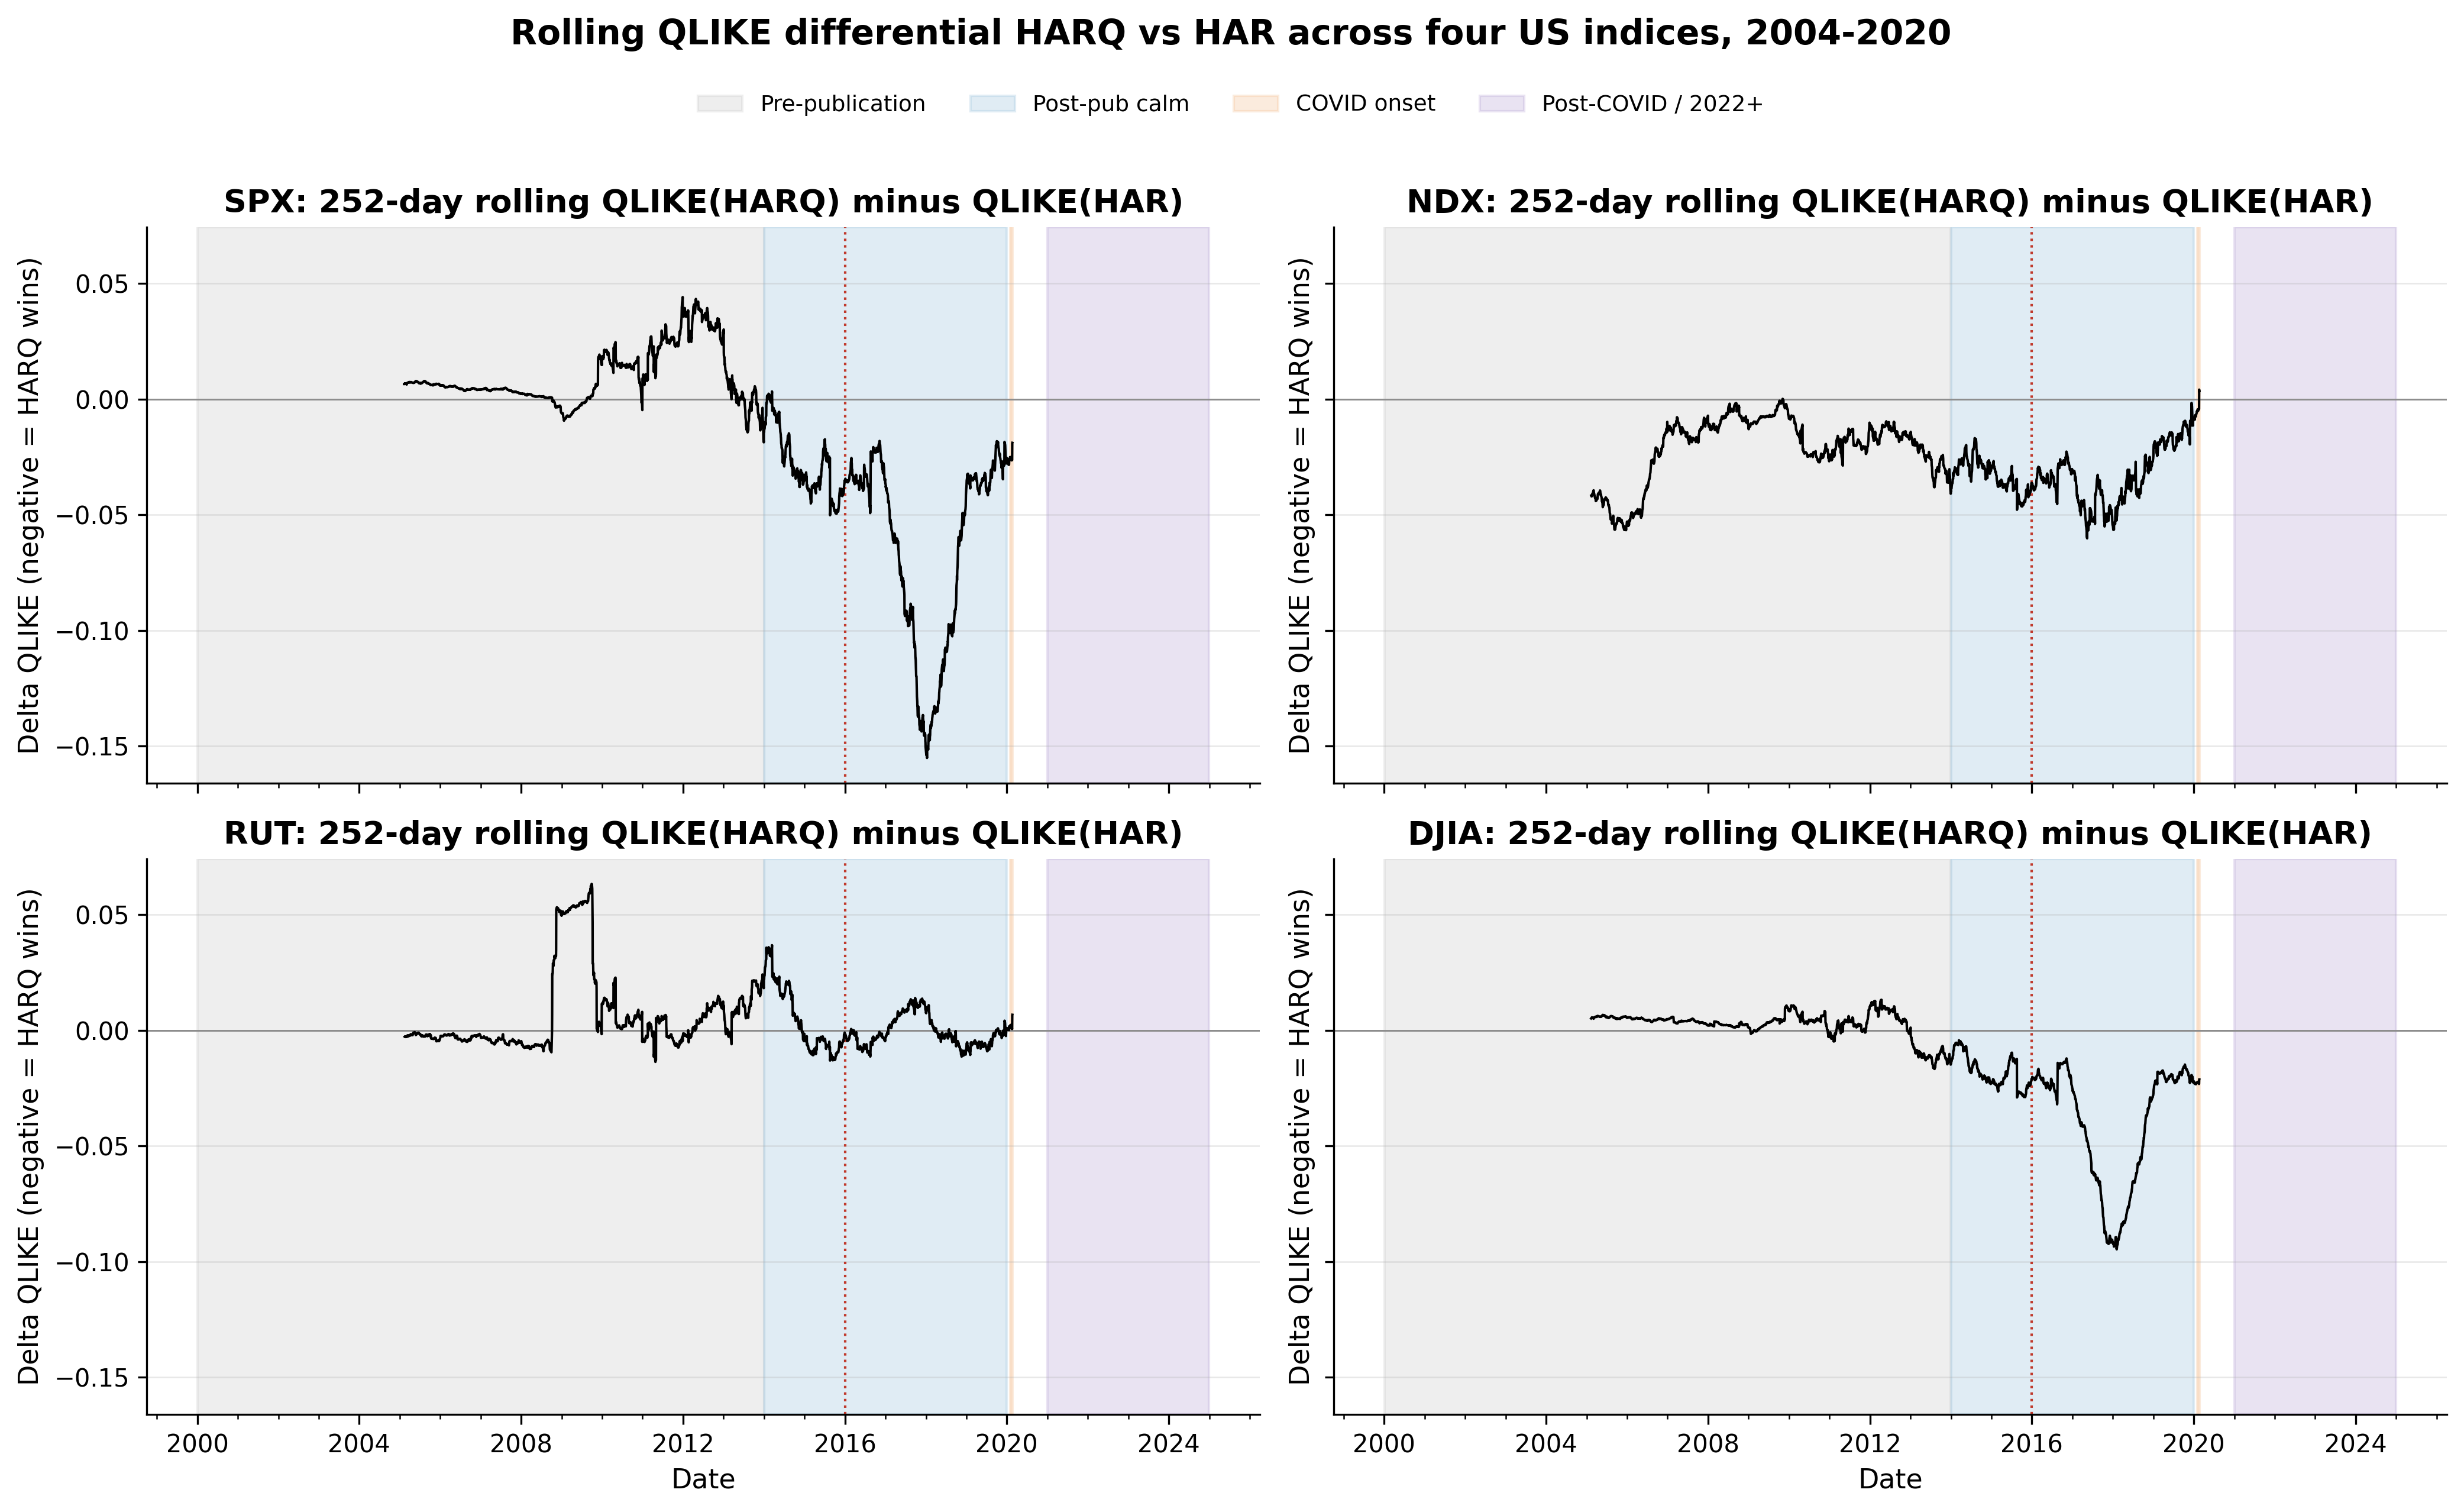
\includegraphics[width=\linewidth]{figures/fig3_rolling_qlike_differential.png}
\caption{Rolling 252-day QLIKE differential $\mathrm{QLIKE}(\text{HARQ}) - \mathrm{QLIKE}(\text{HAR})$ on SPX. Negative = HARQ outperforms HAR; the differential drifts to zero after 2015.}
\label{fig:rolling-qlike}
\end{subfigure}\hfill
\begin{subfigure}{0.48\textwidth}
\centering
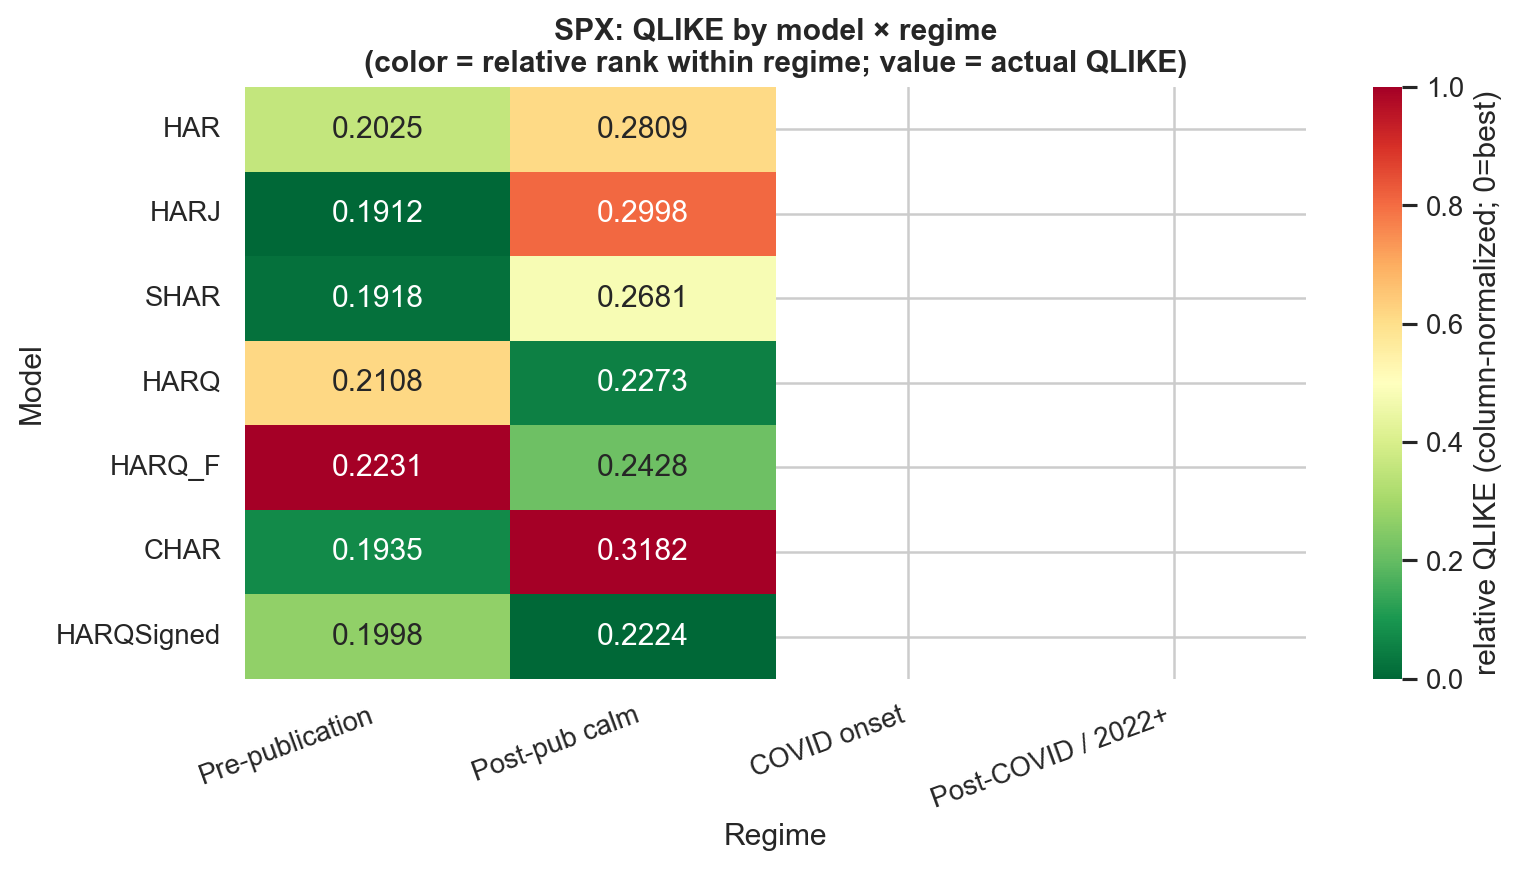
\includegraphics[width=\linewidth]{figures/fig5_regime_heatmap.png}
\caption{SPX QLIKE by model $\times$ regime; colour $=$ QLIKE vs HAR (blue: beats HAR). Grey cells are not evaluable because SHAR / HARQ-Signed require positive/negative semivariances unavailable on SPYRM.}
\label{fig:regime-heatmap}
\end{subfigure}
\end{figure}

\section{Discussion}
\label{sec:discussion}
Three claims survive out-of-sample evaluation on real realized quarticity. First, BPQ's measurement-error correction is real and large in the pre-publication regime --- HARQ-F delivers a 14\% QLIKE reduction on SPX 2002--2013 and the MCS confirms the three HARQ-family models (SHAR, HARQ, HARQ-F) are the only models not significantly worse than the winner. Second, the novel HARQ-Signed specification correctly recovers both the measurement-error sign ($\beta_Q < 0$) and the Patton--Sheppard asymmetry ($\beta_- - \beta_+ \approx +1.1$) in a single regression, and achieves the lowest QLIKE of any model tested on SPX pre-publication. Third, probabilistic volatility forecasting with NGBoost is calibration-viable but still heavy-tail-limited on a Normal output distribution; a follow-up with a Student-$t$ head would be a natural next step. Two findings point to open questions: the post-publication calm regime does not reproduce HARQ's edge --- in the SPY 2014--2019 window HARQ is not statistically better than HAR, and whether this reflects a structural change, an SPY-vs-SPX microstructure artifact, or simply that post-2013 HF data is clean enough that the measurement-error correction offers little remaining signal cannot be resolved without paid SPX HF data through 2024. The crypto null result (HARQ's edge smaller in BTC/ETH than in SPX) similarly invites follow-up at finer sampling on a cleaner exchange-specific sample. The repository is deliberately scoped to assets with genuine realized quarticity; NDX, RUT, DJIA, and the Oxford-Man $BV^2$ proxy were considered and rejected to preserve methodological cleanliness over breadth.

\paragraph{Practical implications.} For a risk desk, the most directly usable finding is NGBoost's near-nominal 96.9\% empirical coverage at the 95\% target: that calibration level is adequate to feed a value-at-risk system, whereas the naive HARQ-plus-Gaussian-residual baseline's 99.5\% over-coverage would systematically under-reserve capital and could mis-size risk buffers. For a quantitative team choosing a model, the rule of thumb that emerges is this: if 5-minute high-frequency data with genuine realized quarticity is available, the HARQ family --- and particularly the new HARQ-Signed specification --- is the right default for in-sample fitting, but out-of-sample in a post-2013 calm regime plain HAR is hard to beat, consistent with declining $RQ$-variation limiting the measurement-error correction's leverage. Finally, the Kupiec rejection at the 1\% VaR tail is a specific warning for future production work: operational volatility-forecasting systems should use a heavy-tailed output distribution (Student-$t$ or Gamma) rather than Normal, because the calibration improvements NGBoost delivers are real but insufficient when the wrong distributional family is fit.

\footnotesize
\setlength{\bibsep}{1pt plus 0.3ex}
\begin{multicols}{2}
\bibliographystyle{abbrvnat}
\bibliography{references}
\end{multicols}

\end{document}
